\documentclass[unicode, notheorems]{beamer}
% is displayed in the header and not the full overview.
\mode<presentation>
{
  \usetheme[numbers, totalnumbers, compress]{Statmod}

  \setbeamercovered{transparent}
  % or whatever (possibly just delete it)
}

%\usepackage{pscyr}
\usepackage[T2A]{fontenc}
\usepackage[utf8]{inputenc}
\usepackage[english,russian]{babel}
\usepackage{xcolor}
\usepackage{amsmath,amssymb,amsfonts,dsfont}
\usepackage{algorithmic}
\usepackage{graphicx,wrapfig}
\ifpdf\usepackage{epstopdf}\fi
%\usepackage{tikz}
% you only need this when using TikZ graphics

\DeclareMathOperator*{\argmax}{arg\,max}
\DeclareMathOperator*{\argmin}{arg\,min}

\graphicspath{{figures/}}

\newtheorem{theorem}{Theorem}
\newtheorem{example}{Example}
\newtheorem{definition}{Definition}

\title{Целевая функций <<QMSE>> для обучения ранжированию}

\author{Сандул Михаил Вадимович, гр. 622}
\institute{Санкт-Петербургский государственный университет \\
    Математико-Механический факультет \\
    Кафедра статистического моделирования \\
    \vspace{0.4cm}
    Научный руководитель: к.ф.-м.н. Шпилёв П.В. \\
    % Место для рецензента \\
    \vspace{0.3cm}
}
\date{
    Санкт-Петербург\\
    2020г.
}

\subject{Beamer}

\begin{document}

\begin{frame}
    \titlepage
\end{frame}

\begin{frame}

\frametitle{Определение задачи ранжирования}

\begin{definition}
Ранжирование --- это процесс упорядочивания объектов по степени их важности, близости к другому объекту или по какому-либо другому критерию
\end{definition}

При этом точное правило неизвестно, или не может быть однозначно выражено с помощью формулы

\end{frame}

\begin{frame}
\frametitle{Пример: IR система}

\begin{figure}[h]
\centering
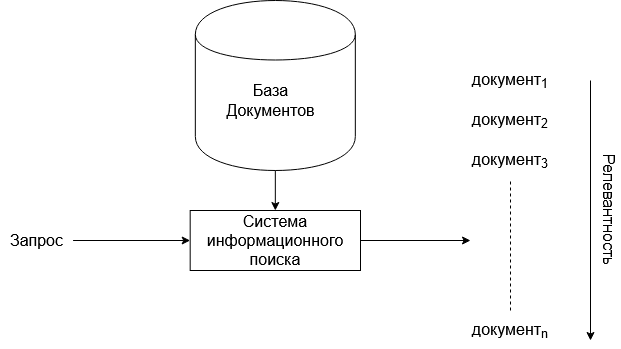
\includegraphics[width=0.7\textwidth]{IRSystem.png}
\label{fig:IRSystem}
\end{figure}

\end{frame}

\begin{frame}

\begin{definition}
Запрос --- фраза на естественном языке, обозначающая то, что хочет найти пользователь
\end{definition}

\begin{definition}
Документ --- объект состоящий из текста, например статья, книга, текстовая часть вэб-страницы
\end{definition}

Документ может иметь структуру, например состоять из параграфов, содержать ссылки на себя или другие документы, иметь заголовок 

\end{frame}

\begin{frame}

\frametitle{Обозначения}

\begin{itemize}
\item $\mathbb Q$ --- множество всех запросов, $q \in \mathbb Q$ --- запрос
\item $\mathbb D$ --- множество всех документов, $d \in \mathbb D$ --- документ
\item $\Phi(q, \{d\}^{n}) = (d_1, d_2, \ldots, d_n)$ --- глобальная ранжирующая функция
\item $\phi(q, d) = r \in \mathbb R$ --- локальная ранжирующая функция
\end{itemize}

\end{frame}


\begin{frame}

\frametitle{Пример локальной ранжирующей функции}

\begin{equation*}
BM25(q, d) = \sum_{t \in q}{\frac{IDF(t) \cdot TF_d(t) \cdot (k_1 + 1)}{TF_d(t) + k_1 \cdot (1 - b + b \cdot \frac{len(d)}{advl})}}
\end{equation*}

\end{frame}

\begin{frame}
\frametitle{Оценка качества: формирование выборки}

\begin{enumerate}
\item $Q = \{q_i\}_{i=1}^{n}$ --- множество случайно отобранных запросов
\item $D_i = \{d_{ij}\}_{j=1}^{m_i}$ --- множество документов, отобранных для запроса $q_i$
\item $L_i = \{l_{ij}\}_{j=1}^{m_j}$ --- метки для документов из множества $D_i$: документу $d_{ij}$  соответствует метка $l_{ij}$
\end{enumerate}

\end{frame}

\begin{frame}
\frametitle{Оценка качества: пример задания меток}

\begin{itemize}
\item Критическая --- речь идет об официальном сайте и официальном ответе на запрос
\item Полезная --- в таком документе можно найти полезную информацию, которая будет четко соответствовать запросу
\item Релевантная$+$ --- документ полностью отвечает на запрос
\item Релевантная$-$ ---документ неточно или неполно отвечает на запрос
\item Не релевантная --- документ не отвечает на запрос
\end{itemize}

\end{frame}

\begin{frame}
\frametitle{Оценка качества: метрика DCG}

\begin{definition}
\begin{equation}
DCG@m(q)=\sum_{i=1}^{m}{G(d_i)\eta(i)},
\end{equation}
\end{definition}
$G(\cdot)$ --- рейтинг документа, рассчитывается по формуле: 

\begin{equation*}
G(\pi^{-1}(i))=G(d_i) = 2^{l_{d_i}} - 1
\end{equation*}

\end{frame}

\begin{frame}
\frametitle{Векторное представление документов}

\begin{itemize}
\item $\{f_i\}_{i=1}^{p}$, $f_i: \mathbb Q \times \mathbb D \rightarrow \mathbb R$ --- локальные ранжирующие функции
\item $F: \mathbb Q \times \mathbb D \rightarrow \mathbb R^p$, $F(q, d) = (f_1(q, d), f_2(q, d), \ldots, f_p(q, d))$ --- векторизующая функция
\item $\mathcal X^j_i = F(q_j, d_i)  = (x^j_{i1}, x^j_{i2}, \ldots x^j_{ip})\in \mathbb R^p$ --- векторное представление пары документ-запрос
\end{itemize}

\end{frame}

\begin{frame}
\frametitle{Обучающая выборка}

\begin{equation*}
\mathbb X =
\begin{pmatrix}
x^1_{1, 1} & x^1_{1, 2} & \cdots & x^1_{1p} \\
x^1_{2, 1} & x^1_{2, 2} & \cdots & x^1_{2p} \\
\vdots & \vdots &  & \vdots \\
x^1_{m_1, 1} & x^1_{m_1, 2} & \ldots & x^1_{m_1, p} \\
\vdots & \vdots &  & \vdots \\
x^n_{1, 1} & x^n_{1, 2} & \cdots & x^n_{1p} \\
x^n_{2, 1} & x^n_{2, 2} & \cdots & x^n_{2p} \\
\vdots & \vdots &  & \vdots \\
x^n_{m_n, 1} & x^n_{m_n, 2} & \cdots & x^n_{m_n, p} \\
\end{pmatrix}\ 
Y =
\begin{pmatrix}
l^1_1 \\
l^1_2 \\
\vdots \\
l^1_{m_1}\\
\vdots \\
l^n_1 \\
l^n_2 \\
\vdots \\
l^n_{m_n}\\
\end{pmatrix}
\end{equation*}

\end{frame}

\begin{frame}
\frametitle{Обучение ранжированию}
\begin{definition}
Локальная ранжирующая функция:
\begin{equation*}
f(\mathcal X^j_i; \Theta) = r
\end{equation*}

$\Theta$ --- вектор неизвестных параметров. Задача: найти оценку $\hat\Theta$ по обучающей выборке $(\mathbb X, Y)$\ 
\end{definition}

\end{frame}

\begin{frame}
\frametitle{Оценка по МНК}

\begin{definition}
\begin{equation*}
\hat\Theta = \argmin_{\tilde\Theta}{\sum_{i=1}^n{\sum_{j=1}^{m_i}{(f(\mathcal X^i_j; \tilde\Theta) - l^i_j) ^ 2}}}
\end{equation*}
\end{definition}

MSE --- это оценка сверху для NDCG:
\begin{equation*}
1 - NDCG(f, \mathbb X, Y) \leq \frac{1}{Z_m}\Big( 2 \sum_{j=1}^{m}{\eta(j)^2}\Big)^{\frac{1}{2}} \Big( \sum_{j=1}^{m}{(f(\mathcal X_j) - l_j)^2}\Big)^{\frac{1}{2}}\,
\end{equation*}

\end{frame}

\begin{frame}
\frametitle{Формулировка задачи}

У MSE есть ряд недостатков:

\begin{itemize}
\item Не учитывает разбиение по запросам
\item Не учитывает специфику задачи: значения $r$ должны задавать правильный порядок, но могут не совпадать с метками
\end{itemize}

Наша задача состоит в том, чтобы  построить функцию потерь, которая не будет иметь таких недостатков

\end{frame}

\begin{frame}
\frametitle{Функция потерь QMSE}

\begin{definition}
\begin{equation*}
QMSE = \sum_{i=1}^{n}{\sum_{j=1}^{m_i}{\big(  l^i_j - f(\mathcal X^i_j; \Theta)) - m_i \big)^2}}
\end{equation*}
\end{definition}
Где $m_i = \frac{1}{m_i}\sum_{k=1}^{m_i}{l^i_j - f(\mathcal X^i_k; \Theta)}$

\end{frame}

\begin{frame}
\frametitle{Свойства QMSE: градиент}

Введем обозначения:
\begin{itemize}
\item $s^i_j  = f(\mathcal X^i_j; \Theta)$ 
\item $E_{ij} = l^i_j - s^i_j -  \frac{1}{m_i}\sum_{k=1}^{m_i}{l^i_j - s^i_j}$
\end{itemize}

Тогда:
\begin{equation*}
\nabla_s (QMSE(l, s)) = -2 (E_{11}, E_{12}, \ldots, E_{1,m_1}, \ldots, E_{n1}, E_{n2}, \ldots, E_{nm_n})
\end{equation*}

\end{frame}

\begin{frame}
\frametitle{Свойства QMSE: устойчивость к сдвигу}
Рассмотрим ошибку $E_{ij}$:

\begin{equation*}
\begin{split}
E_{ij} & =  l^i_j - s^i_j -  \frac{1}{m_i}\sum_{k=1}^{m_i}{l^i_j - s^i_j} = \\ & = \frac{1}{m_i}\sum_{k=1}^{m_i}{(l^i_j - l^i_k) - (s^i_j - s^i_k)} = \\ & = \frac{1}{m_i}\sum_{k=1}^{m_i}{(l^i_j - l^i_k)} - \frac{1}{m_i}\sum_{k=1}^{m_i}{(s^i_j - s^i_k)}
\end{split}
\end{equation*}

\end{frame}

\end{document}